%%%%%%%%%%%%%%%%%%%%%%%%%%%%%%%%%%%%%%%%%
% Lachaise Assignment
% LaTeX Template
% Version 1.0 (26/6/2018)
%
% This template originates from:
% http://www.LaTeXTemplates.com
%
% Authors:
% Marion Lachaise & François Févotte
% Vel (vel@LaTeXTemplates.com)
%
% License:
% CC BY-NC-SA 3.0 (http://creativecommons.org/licenses/by-nc-sa/3.0/)
% 
%%%%%%%%%%%%%%%%%%%%%%%%%%%%%%%%%%%%%%%%%

%----------------------------------------------------------------------------------------
%	PACKAGES AND OTHER DOCUMENT CONFIGURATIONS
%----------------------------------------------------------------------------------------

\documentclass{article}

%%%%%%%%%%%%%%%%%%%%%%%%%%%%%%%%%%%%%%%%%
% Lachaise Assignment
% Structure Specification File
% Version 1.0 (26/6/2018)
%
% This template originates from:
% http://www.LaTeXTemplates.com
%
% Authors:
% Marion Lachaise & François Févotte
% Vel (vel@LaTeXTemplates.com)
%
% License:
% CC BY-NC-SA 3.0 (http://creativecommons.org/licenses/by-nc-sa/3.0/)
% 
%%%%%%%%%%%%%%%%%%%%%%%%%%%%%%%%%%%%%%%%%

%----------------------------------------------------------------------------------------
%	PACKAGES AND OTHER DOCUMENT CONFIGURATIONS
%----------------------------------------------------------------------------------------

\usepackage{dirtree}
\usepackage{float} % here for H placement parameter
\usepackage{amsmath,amsfonts,stmaryrd,amssymb} % Math packages
\usepackage[dvipsnames]{xcolor}
\usepackage{enumerate} % Custom item numbers for enumerations
\usepackage{hyperref}
%\usepackage[ruled,vlined]{algorithm2e} % Algorithms
\usepackage{algpseudocode}
\usepackage{algorithm}
\usepackage[framemethod=tikz]{mdframed} % Allows defining custom boxed/framed environments

\usepackage{listings} % Required for insertion of code

\newcommand{\randomcolor}{%
  \definecolor{randomcolor}{RGB}
   {
    \pdfuniformdeviate 256,
    \pdfuniformdeviate 256,
    \pdfuniformdeviate 256
   }%
  \color{randomcolor}%
}

\definecolor{codegreen}{rgb}{0,0.6,0}
\definecolor{codegray}{rgb}{0.5,0.5,0.5}
\definecolor{codepurple}{rgb}{0.58,0,0.82}
\definecolor{backcolour}{rgb}{1,1,1}
\lstdefinestyle{mystyle}{
    backgroundcolor=\color{backcolour},   
    commentstyle=\color{codegreen},
    keywordstyle=\color{magenta},
    numberstyle=\tiny\color{codegray},
    stringstyle=\color{codepurple},
    basicstyle=\ttfamily\footnotesize,
    breakatwhitespace=false,         
    breaklines=true,                 
    captionpos=b,                    
    keepspaces=true,                 
    numbers=left,                    
    numbersep=5pt,                  
    showspaces=false,                
    showstringspaces=false,
    showtabs=false,                  
    tabsize=2
}
\renewcommand{\lstlistingname}{Código}% Listing -> Algorithm
\lstset{style=mystyle}


%\usepackage{listings} % File listings, with syntax highlighting
%\lstset{
%	basicstyle=\ttfamily, % Typeset listings in monospace font
%}

%----------------------------------------------------------------------------------------
%	DOCUMENT MARGINS
%----------------------------------------------------------------------------------------

\usepackage{geometry} % Required for adjusting page dimensions and margins

\geometry{
	paper=a4paper, % Paper size, change to letterpaper for US letter size
	top=2.5cm, % Top margin
	bottom=3cm, % Bottom margin
	left=2.5cm, % Left margin
	right=2.5cm, % Right margin
	headheight=14pt, % Header height
	footskip=1.5cm, % Space from the bottom margin to the baseline of the footer
	headsep=1.2cm, % Space from the top margin to the baseline of the header
	%showframe, % Uncomment to show how the type block is set on the page
}

%----------------------------------------------------------------------------------------
%	FONTS
%----------------------------------------------------------------------------------------

\usepackage[utf8]{inputenc} % Required for inputting international characters
\usepackage[T1]{fontenc} % Output font encoding for international characters

\usepackage{XCharter} % Use the XCharter fonts

%----------------------------------------------------------------------------------------
%	COMMAND LINE ENVIRONMENT
%----------------------------------------------------------------------------------------

% Usage:
% \begin{commandline}
%	\begin{verbatim}
%		$ ls
%		
%		Applications	Desktop	...
%	\end{verbatim}
% \end{commandline}

\mdfdefinestyle{commandline}{
	leftmargin=10pt,
	rightmargin=10pt,
	innerleftmargin=15pt,
	middlelinecolor=black!50!white,
	middlelinewidth=2pt,
	frametitlerule=false,
	backgroundcolor=black!5!white,
	frametitle={Command Line},
	frametitlefont={\normalfont\sffamily\color{white}\hspace{-1em}},
	frametitlebackgroundcolor=black!50!white,
	nobreak,
}

% Define a custom environment for command-line snapshots
\newenvironment{commandline}{
	\medskip
	\begin{mdframed}[style=commandline]
}{
	\end{mdframed}
	\medskip
}

%----------------------------------------------------------------------------------------
%	FILE CONTENTS ENVIRONMENT
%----------------------------------------------------------------------------------------

% Usage:
% \begin{file}[optional filename, defaults to "File"]
%	File contents, for example, with a listings environment
% \end{file}

\mdfdefinestyle{file}{
	innertopmargin=1.6\baselineskip,
	innerbottommargin=0.8\baselineskip,
	topline=false, bottomline=false,
	leftline=false, rightline=false,
	leftmargin=2cm,
	rightmargin=2cm,
	singleextra={%
		\draw[fill=black!10!white](P)++(0,-1.2em)rectangle(P-|O);
		\node[anchor=north west]
		at(P-|O){\ttfamily\mdfilename};
		%
		\def\l{3em}
		\draw(O-|P)++(-\l,0)--++(\l,\l)--(P)--(P-|O)--(O)--cycle;
		\draw(O-|P)++(-\l,0)--++(0,\l)--++(\l,0);
	},
	nobreak,
}

% Define a custom environment for file contents
\newenvironment{file}[1][File]{ % Set the default filename to "File"
	\medskip
	\newcommand{\mdfilename}{#1}
	\begin{mdframed}[style=file]
}{
	\end{mdframed}
	\medskip
}

%----------------------------------------------------------------------------------------
%	NUMBERED QUESTIONS ENVIRONMENT
%----------------------------------------------------------------------------------------

% Usage:
% \begin{question}[optional title]
%	Question contents
% \end{question}

\mdfdefinestyle{question}{
	innertopmargin=1.2\baselineskip,
	innerbottommargin=0.8\baselineskip,
	roundcorner=5pt,
	nobreak,
	singleextra={%
		\draw(P-|O)node[xshift=1em,anchor=west,fill=white,draw,rounded corners=5pt]{%
		Pregunta \theQuestion\questionTitle};
	},
}

\newcounter{Question} % Stores the current question number that gets iterated with each new question

% Define a custom environment for numbered questions
\newenvironment{question}[1][\unskip]{
	\bigskip
	\stepcounter{Question}
	\newcommand{\questionTitle}{~#1}
	\begin{mdframed}[style=question]
}{
	\end{mdframed}
	\medskip
}

%----------------------------------------------------------------------------------------
%	WARNING TEXT ENVIRONMENT
%----------------------------------------------------------------------------------------

% Usage:
% \begin{warn}[optional title, defaults to "Warning:"]
%	Contents
% \end{warn}

\mdfdefinestyle{warning}{
	topline=false, bottomline=false,
	leftline=false, rightline=false,
	nobreak,
	singleextra={%
		\draw(P-|O)++(-0.5em,0)node(tmp1){};
		\draw(P-|O)++(0.5em,0)node(tmp2){};
		\fill[black,rotate around={45:(P-|O)}](tmp1)rectangle(tmp2);
		\node at(P-|O){\color{white}\scriptsize\bf !};
		\draw[very thick](P-|O)++(0,-1em)--(O);%--(O-|P);
	}
}

% Define a custom environment for warning text
\newenvironment{warn}[1][Warning:]{ % Set the default warning to "Warning:"
	\medskip
	\begin{mdframed}[style=warning]
		\noindent{\textbf{#1}}
}{
	\end{mdframed}
}

%----------------------------------------------------------------------------------------
%	INFORMATION ENVIRONMENT
%----------------------------------------------------------------------------------------

% Usage:
% \begin{info}[optional title, defaults to "Info:"]
% 	contents
% 	\end{info}

\mdfdefinestyle{info}{%
	topline=false, bottomline=false,
	leftline=false, rightline=false,
	nobreak,
	singleextra={%
		\fill[black](P-|O)circle[radius=0.4em];
		\node at(P-|O){\color{white}\scriptsize\bf i};
		\draw[very thick](P-|O)++(0,-0.8em)--(O);%--(O-|P);
	}
}

% Define a custom environment for information
\newenvironment{info}[1][Info:]{ % Set the default title to "Info:"
	\medskip
	\begin{mdframed}[style=info]
		\noindent{\textbf{#1}}
}{
	\end{mdframed}
}
 % Include the file specifying the document structure and custom commands

%----------------------------------------------------------------------------------------
%	ASSIGNMENT INFORMATION
%----------------------------------------------------------------------------------------

\title{IC-2023: Tarea \#1} % Title of the assignment

\author{Luis Ballado\\ \texttt{luis.ballado@cinvestav.mx}} % Author name and email address

\date{CINVESTAV UNIDAD TAMAULIPAS --- \today} % University, school and/or department name(s) and a date

%----------------------------------------------------------------------------------------
\algnewcommand\algorithmicforeach{\textbf{for each}}
\algdef{S}[FOR]{ForEach}[1]{\algorithmicforeach\ #1\ \algorithmicdo}

\begin{document}

\maketitle % Print the title

%----------------------------------------------------------------------------------------
%	INTRODUCTION
%----------------------------------------------------------------------------------------

\section{Instrucciones para ejecución}

\begin{info} % Information block
  Se adjunta la liga al repositorio, donde se encuentran todos los códigos\\
  \href{https://github.com/luisballado/InteligenciaComputacional/tree/master/code/tarea1}{ver código en github}\\
\end{info}

\begin{info} % Information block
  Se hacen uso de las siguientes bibliotecas de Python
  \begin{itemize}
  \item numpy  - manejo de vectores, cálculos vectoriales, normalizar, aleatoriedad
  \item random - aleatoriedad
  \item abc - creación de clases abstractas
  \item matplotlib - generación de gráficos mostrados en las estadisticas
  \item pandas - para los programas de resultados y calculos de media, desviación std.
  \item scipy - para los programas de resultados y calculos de media, desviación std. 
  \end{itemize}
\end{info}

\begin{enumerate} 

\item Clonar el repositorio
  
\begin{commandline}
 \begin{verbatim}
  $ git clone https://github.com/luisballado/InteligenciaComputacional.git
  $ cd InteligenciaComputacional
  $ cd code
  $ cd tarea1
 \end{verbatim}
\end{commandline}

\newpage
\item Descripción Archivos \\

  Dentro del repositorio se sigue la siguiente estructura para organizar los archivos por paradigma genetico como se muestra:\\
  
  \dirtree{%
    .1 tarea1/.
    .2 DE.
    .3 EvolucionDiferencial.py.
    .3 test\_differential\_evolution.py.
    .3 resultados.
    .4 resultado\_graficos.py.
    .4 resultados\_globales.py.
    .4 resultados.py.
    .4 resultados.txt.
    .2 EP.
    .3 ProgramacionEvolutiva.py.
    .3 test\_evolution\_programming.py.
    .3 resultado\_graficos.py.
    .3 resultados.py.
    .3 rosen\_results/.
    .4 resultado\_global.txt.
    .3 sphere\_results/.
    .4 resultado\_global.txt.
    .3 ackley.
    .4 resultado\_global.txt.
    .2 ES.
    .3 EstrategiasEvolutivas.py.
    .3 test\_evolution\_estrategies.py.
    .3 resultado\_ackley.txt.
    .3 resultado\_esfera.txt.
    .3 resultado\_graficos.py.
    .3 resultado.py.
    .3 resultado\_rosen.txt.
    .3 resultados\_globales.txt.
  }

\end{enumerate} 

%---------------------------------------------------------------------

\newpage
\section{Programación Evolutiva}

\subsection{Pseudocódigo}
\begin{algorithm} \caption{Pseudocódigo Programación Evolutiva}
  \begin{algorithmic}[1]
    \State Inicializar el número de generaciones a 0 $(t=0)$
    \State Inicializar la población P de N individuos con valores aleatorios
    \State Evaluar la aptitud de cada individuo en la Población
    \Repeat
    \State Ordenar la población P en orden decreciente de aptitud
    \State Calcular la tasa de éxito SR = (número de mutaciones exitosas) / (número total de mutaciones)
    \If {$SR > 1/5$}
    \State aumentar $\sigma$ por un factor de $e(1/4)$
    \Else
    \State disminuir $\sigma$ por un factor de $e(-1/4)$
    \EndIf
    \If {$SR < 1/5$}
    \State disminuir $\mu$ por un factor de $e(-1/4)$
    \Else
    \State aumentar $\mu$ por un factor de $e(1/4)$
    \EndIf
    \State Generar una nueva población P' de N individuos con los siguientes pasos:
    \begin{itemize}
    \item Seleccionar dos padres utilizando la selección de torneos
    \item Generar un nuevo individuo agregando una perturbación distribuida normalmente al promedio ponderado de los dos padres
    \item Evaluar la aptitud del nuevo individuo
    \end{itemize}
    \State Reemplazar el peor individuo en P con el mejor individuo en P'
    \Until {se cumpla el criterio de parada}
    \State Seleccionar el mejor individuo de la Población(P) como solución
  \end{algorithmic}
\end{algorithm}

En este algoritmo, N es el tamaño de la población, $\sigma$ es la desviación estándar de la distribución normal y $\mu$ es la tasa de mutación. \\La selección de torneos se realiza seleccionando aleatoriamente cuatro individuos y seleccionando los dos mejores según su aptitud. \\El criterio de parada puede basarse en el número de evaluaciones de función, la convergencia de la solución o un número máximo de iteraciones.\\

La regla 1/5 se utiliza para adaptar las tasas de mutación y perturbación en respuesta a la tasa de éxito del algoritmo. \\Si la tasa de éxito es alta, las tasas de mutación y perturbación se aumentan y si es baja, se disminuyen. Esto ayuda a mantener un equilibrio entre la exploración y la explotación en el proceso de búsqueda.\\

\begin{enumerate} 
\item Ejecutar Programacion Evolutiva
  \href{https://github.com/luisballado/InteligenciaComputacional/tree/master/code/tarea1/EP}{ver código en github}\\
  \begin{enumerate}
  \item entrar a la carpeta EP
  \item correr el programa test\_evolution\_programming.py 100000 21 1234 10 4
  \end{enumerate} 
  
  Los siguientes comando hacen lo descrito arriba, donde se le pasa como argumentos: max\_iteraciones, num\_poblacion, semilla, dimension, num\_torneos
  
  \begin{commandline}
     \begin{verbatim}
    $ cd EP       
    $ python3.10 test_evolution_programming.py 100000 21 1234 10 4
     \end{verbatim}
  \end{commandline}
  
  Ejemplo de resultados:
  
  \begin{commandline}
     \begin{verbatim}
       $ python3.10 test_evolution_programming.py 100000 21 1234 10 4
       #######ESFERA########
       Minimo Esfera - 0.002827846527436945
       Tiempo - 1.0355191230773926 segundos
       #######ACKLEY########
       Minimo - 6.921701528961158
       Tiempo - 2.3101282119750977 segundos
       #######ROSENBROCK########
       Minimo ROSENBROCK - 0.011268231197750245
       Tiempo - 1.9178040027618408 segundos

     \end{verbatim}
  \end{commandline}
  
\end{enumerate} 

%---------------------------------------------------------------------

\newpage
\section{Estrategias Evolutivas}
\subsection{Pseudocódigo}

\begin{algorithm} \caption{Pseudocódigo Estrategias Evolutivas}
  \begin{algorithmic}[1]
    \State Inicializar el número de generaciones a 0 $(t=0)$
    \State Inicializar la población de $\mu$ individuos en la población P
    \State Evaluar la aptitud de cada individuo en la población P
    \Repeat
    \State t=t+1
    \If {estrategia comma}
    \State generar $\lambda$ descendientes por cada padre de $\mu$ seleccionando dos padres y generando una perturbación distribuida normalmente a la media ponderada de los padres.
    \EndIf
    \If {estrategia plus}
    \State generar $\lambda$ descendientes seleccionando $\lambda$ padres aleatorios y generando una perturbación distribuida normalmente a la media ponderada de los padres.
    \EndIf
    \State Unir la población mu y la descendencia lambda y seleccionar los mu mejores individuos (estrategia comma) o seleccionar los mu individuos únicos de la población mu y descendencia lambda (estrategia plus).
    \State Calcular la tasa de éxito SR = (número de mutaciones exitosas) / (número total de mutaciones)
    \If{$SR > 1/5$}
    \State aumentar sigma por un factor de $e(1/4)$
    \Else
    \State disminuir sigma por un factor de $e(-1/4)$
    \EndIf
    \If{$SR < 1/5$}
    \State disminuir mu por un factor de $e(-1/4)$
    \Else
    \State aumentar mu por un factor de $e(1/4)$
    \EndIf
    \Until {hasta que se cumpla el criterio de parada}
    \State Seleccionar el mejor individuo de la Población como solución
  \end{algorithmic}
\end{algorithm}

En este algoritmo, $\mu$ es el tamaño de la población de padres, $\lambda$ es el tamaño de la población de descendencia, sigma es la desviación estándar de la distribución normal y $\mu$ es la tasa de mutación. La selección de padres se realiza seleccionando los mejores $\mu$ individuos para las estrategias de coma y seleccionando aleatoriamente $\lambda$ individuos para las estrategias de suma. La regla 1/5 se utiliza para adaptar las tasas de mutación y perturbación de manera similar a la Programación Evolutiva.

\begin{enumerate} 
\item Ejecutar Estrategias Evolutivas
  \href{https://github.com/luisballado/InteligenciaComputacional/tree/master/code/tarea1/ES}{ver código en github}\\
  \begin{enumerate}
  \item entrar a la carpeta ES \\
  \item correr el programa test\_evolution\_estrategies.py\\
  \end{enumerate} 

  Los siguientes comando hacen lo descrito arriba, donde se le pasa como argumentos: max\_iteraciones, dimension, semilla, tam\_poblacion

  \begin{commandline}
     \begin{verbatim}
        $ cd ES
        $ python3.10 test_evolution_estrategies.py 1000 10 123 21
     \end{verbatim}
  \end{commandline}

  Ejemplo de resultados:
  % Command-line "screenshot"
  \begin{commandline}
\begin{verbatim}
  $ python3.10 test_evolution_estrategies.py 1000 10 123 21
  #######ESFERA########
  Minimo Esfera - 0.0030510694905647798
  Tiempo - 9.76209020614624 segundos
  #######ACKLEY########
  Minimo - 2.9760964277078257
  Tiempo - 22.16294836997986 segundos
  #######ROSENBROCK########
  Minimo ROSENBROCK - 0.5528162673457115
  Tiempo - 18.074426412582397 segundos
  
\end{verbatim}
  \end{commandline}
\end{enumerate}

%---------------------------------------------------------------------

\newpage
\section{Evolucion Diferencial}
\subsection{Pseudocódigo}

\begin{algorithm} \caption{Pseudocódigo Evolución Diferencial}
  \begin{algorithmic}[1]
    \Require tam\_poblacion, factor de mutación(F), factor de cruza(CR)
    \State Asignar el número de generaciones a 0 ($t=0$)
    \State Inicializar la población P, con el tam\_población
    \State Evaluar el fitness de cada individuo de la Población P
    \Repeat
    \State $t=t+1$
    \ForEach {$individuo \in \mathcal P $}
    \State Seleccionar tres diferentes indivuduos de P que sean diferentes: $r1\neq X2 \neq X3 \in P$
    \ForEach {$j-th$ gene $\in individuo $}
    \State $v_{i,j} = x_{r1,j} + F * (x_{r2,j}-x{r3,j})$
    \State generar un número aleatorio $rand_{j} \in \mathcal 0;1$
    \If {$rand_{j} < CR$}
    \State $u_{i,j} := v_{i,j}$
    \Else
    \State $u_{i,j}:=x_{i,j}$
    \EndIf
    \EndFor
    \If{$individuo u_{i} es mejor que el individuo x_{i}$}
    \State remplazar el individuo $x_i$ por el elemento del vector en $u_{i}$
    \EndIf
    \EndFor
    \Until {hasta que se cumpla el criterio de parada}
    \State Seleccionar el mejor individuo de la Población(P) como solución
  \end{algorithmic}
\end{algorithm}

\begin{enumerate}
  \item Ejecutar Evolución Diferencial
    \href{https://github.com/luisballado/InteligenciaComputacional/tree/master/code/tarea1/DE}{ver código en github}\\
    \begin{enumerate}
    \item entrar a la carpeta DE \\
    \item correr el programa test\_differential\_evolution.py\\
    \end{enumerate} 

    Los siguientes comando hacen lo descrito arriba, donde se le pasa como argumentos: max\_iteraciones, tam\_poblacion, semilla, dimension
    
    \begin{commandline}
\begin{verbatim}
  $ cd DE
  $ python3.10 test_differential_evolution.py 1000 21 1234 10 0.7 0.8
\end{verbatim}
    \end{commandline}

    Ejemplo de resultados:

    \begin{commandline}
\begin{verbatim}
  $ python3.10 test_differential_evolution.py 1000 21 1234 10 0.7 0.8
  #######ESFERA########
  Minimo Esfera - 0.32934544659126797
  Tiempo - 0.9660787582397461 segundos
  #######ACKLEY########
  Minimo - 5.653204234520572
  Tiempo - 1.2940564155578613 segundos
  #######ROSENBROCK########
  Minimo ROSENBROCK - 0.27512093701771834
  Tiempo - 1.1127583980560303 segundos
\end{verbatim}
    \end{commandline}
\end{enumerate} 

\section{Decisiones de implementación}

El código hace uso de NumPy arrays en su mayoria para representar vectores y matrices que son el tipo de estructura de datos convenientes para los calculos y fácil manipulación que nos brinda la libreria.\\

Todos los paradigmas los englobe en clases para tener un mejor control de ellas y poder iterar en la evaluación de sus diferentes funciones objetivo.\\

Se usan diferentes tipos de variables que python internamente interpretará como de tipo entero o flotante como las empleadas para el número de iteraciones, tamaño de poblacion, dimesiónes del problema, limites máx-min, objetos de tipo funciones para pasarlas a las clases

Los módulos de random son también usados para crear números random para la generaciones de poblaciones.\\

En teoría, es posible implementar los algoritmos de programación evolutiva, estrategias evolutivas y evolución diferencial utilizando la recursión, pero generalmente no se hace ya que en generaciones grandes se puede llegar al limite y desbordar el stack. Las implementaciones utilizan estructuras de bucles iterativos para mejorar la eficiencia y la claridad del código. 
\newpage
\section{Estadisticas}
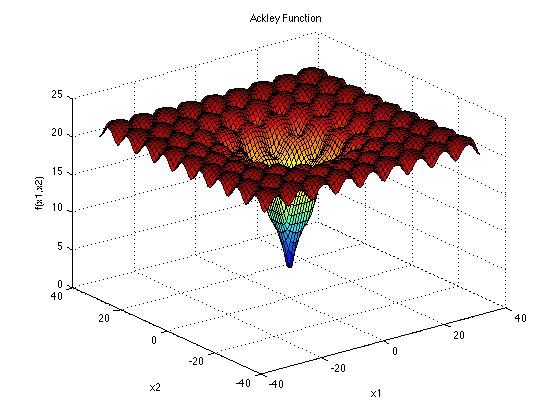
\includegraphics[scale=0.3]{ackley.png}
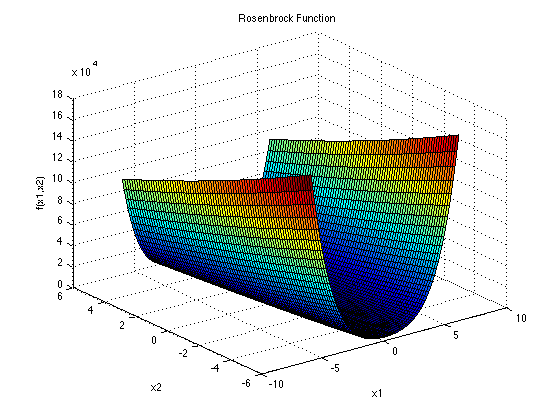
\includegraphics[scale=0.3]{rosen.png}
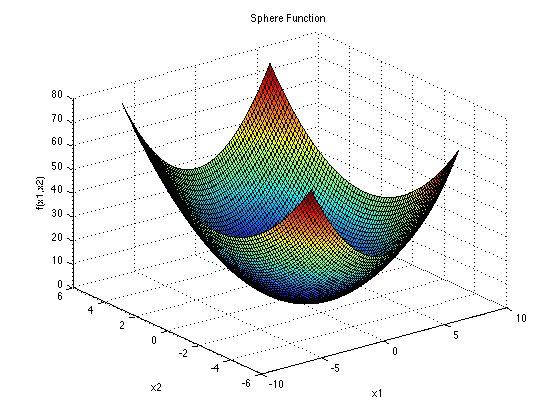
\includegraphics[scale=0.3]{sphere.png}

Se crearon dos programas para la generación de los gráficos y los cálculos estadísticos con ayuda de las librerias matplotlib.\\
Los archivos se encuentran en las respectivas carpetas para cada paradigma genético

\begin{itemize}
\item resultado\_graficos.py
\item resultados.py
\end{itemize}

\subsection{Evolución Diferencial}
\begin{table}[H]
  \centering
  \begin{tabular}{|l|l|l|l|}
    \hline
        {\textit{\textbf{DE}}} & ESFERA   & ACKLEY   & ROSENBROCK \\ \hline
        min                        & 0.000294 & 0.017313 & 0.022593   \\ \hline
        mean                       & 0.537641 & 0.421045 & 0.536638   \\ \hline
        std                        & 0.672198 & 0.413683 & 0.405818   \\ \hline
  \end{tabular}
\end{table}

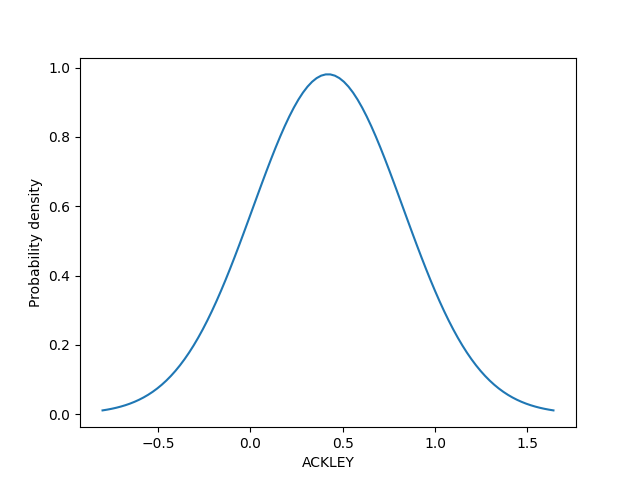
\includegraphics[scale=0.5]{DE/ackley.png}
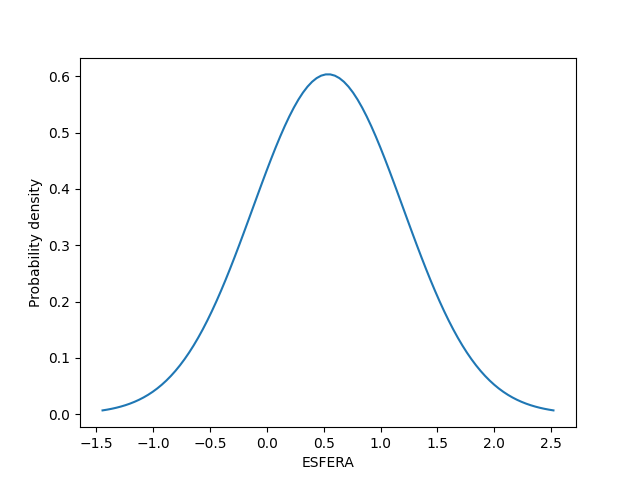
\includegraphics[scale=0.5]{DE/esfera.png}
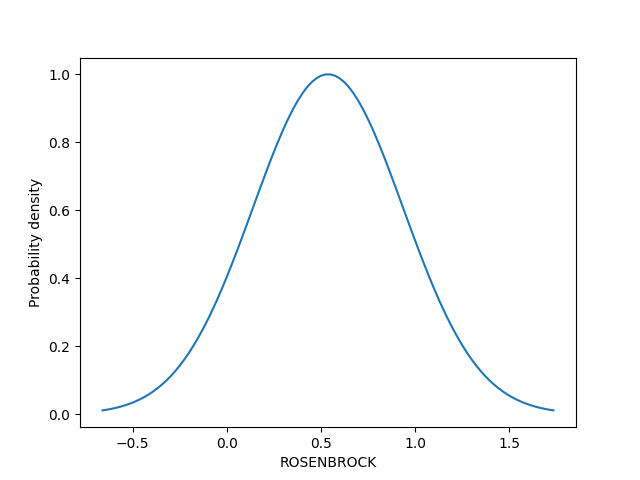
\includegraphics[scale=0.5]{DE/rosenbrock.png}


\newpage
\subsection{Programación Evolutiva}
\begin{table}[H]
  \centering
  \begin{tabular}{|l|l|l|l|}
    \hline
    \textit{\textbf{EP}} & ESFERA   & ACKLEY   & ROSENBROCK \\ \hline
    min                  & 0.000005 & 0.000179 & 0.250946   \\ \hline
    mean                 & 0.001134 & 0.46137  & 0.396463   \\ \hline
    std                  & 0.001057 & 0.562699 & 0.060919   \\ \hline
  \end{tabular}
\end{table}

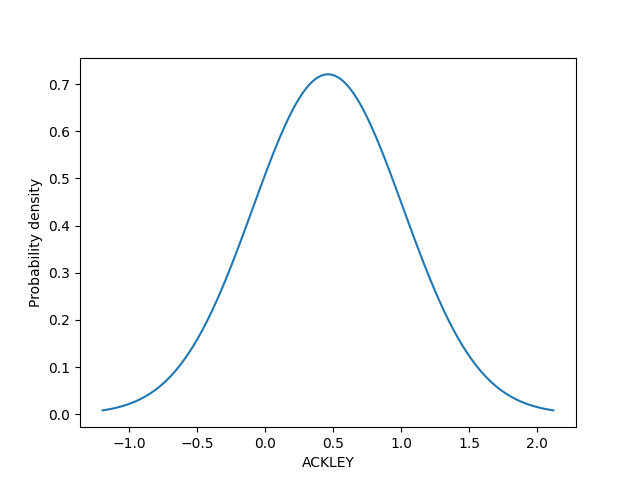
\includegraphics[scale=0.5]{EP/ackley.png}
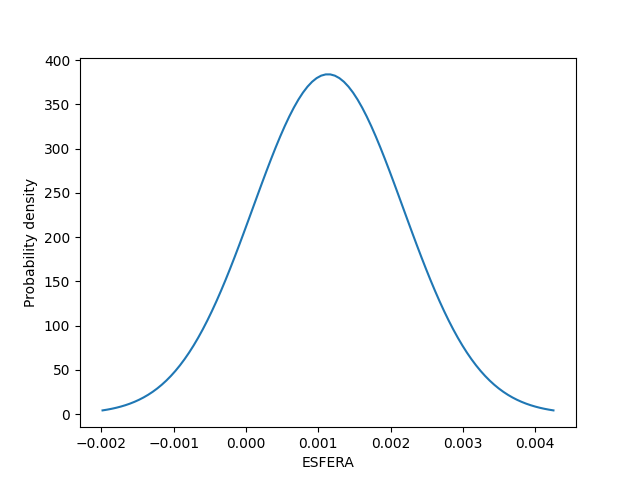
\includegraphics[scale=0.5]{EP/esfera.png}
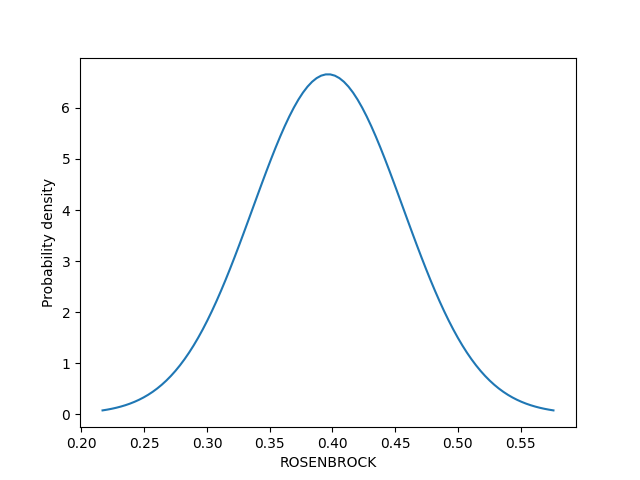
\includegraphics[scale=0.5]{EP/rosenbrock.png}

\newpage
\subsection{Estrategias Evolutivas}
\begin{table}[H]
  \centering
  \begin{tabular}{|l|l|l|l|}
    \hline
    \textit{\textbf{ES}} & ESFERA   & ACKLEY   & ROSENBROCK \\ \hline
    min                  & 0.003511 & 0.001876 & 0.005112   \\ \hline
    mean                 & 0.132062 & 0.111832 & 0.16726    \\ \hline
    std                  & 0.14831  & 0.086868 & 0.20306    \\ \hline
  \end{tabular}
\end{table}

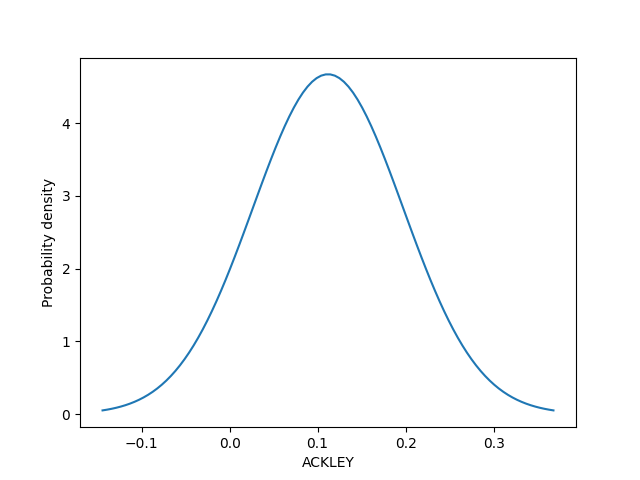
\includegraphics[scale=0.5]{ES/ackley.png}
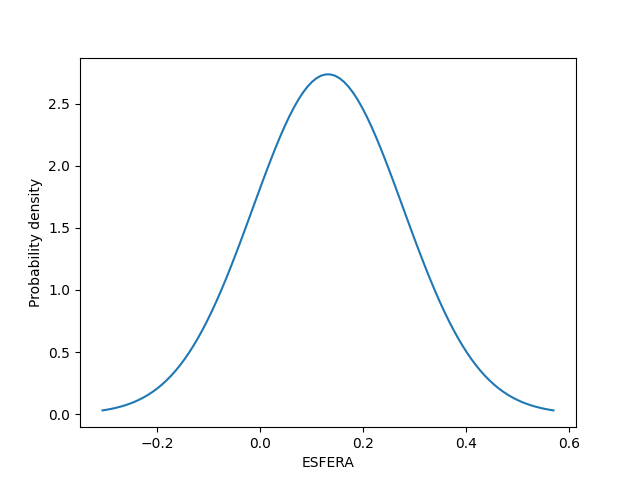
\includegraphics[scale=0.5]{ES/esfera.png}
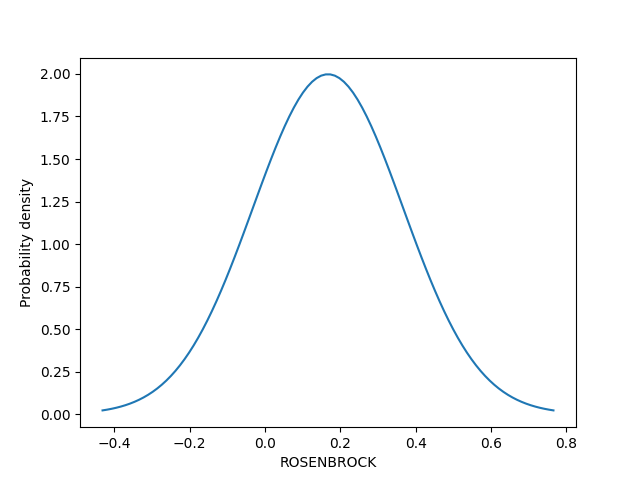
\includegraphics[scale=0.5]{ES/rosenbrock.png}


\section{Conclusiones}

Durante las corridas se observaron las diferentes soluciones ya que el proceso de optimización es estocástico, lo que involucra aleatoriedad lo que hace que los diferentes algoritmos encuentren diferentes soluciones para cada corrida y es posible que para multiples soluciones sean igual de buenas (que tengan el mismo valor minimo).\\

La elección de cuál algoritmo es mejor de usar para una función objetivo en particular, depende de varios factores como la estructura del problema. Al incio me fué complicado entender como podría crear las funciones objetivos y que es lo que se buscaba realmente, pero mientras más me adentraba al tema pude entender que al final del dia es una función limitada en un rango donde existe un mínimo o un máximo global y en ocasiones solo encontramos los mínimos locales y es importando tener un cambio de factor de mutación para poder ir saliendo de estos mínimos e ir buscando los globales.\\

No hay un mejor o peor algoritmo, todos tienen sus fortalezas y debilidades, Programacion Evolutiva (EP), Estrategias Evolutivas (ES) y Evolución Diferencial (DE) todos son metahuristicas de optimización que pertenecen a la familia de técnicas de Computación Evolutiva\\

\end{document}

